%! Author = loreb
%! Date = 31/10/2023

% Preamble
\documentclass[11pt]{article}

% Packages
\usepackage{amsmath}
\usepackage{graphicx}
\usepackage{float}
\usepackage{csvsimple}
\usepackage{hyperref}
\usepackage{listings}
\usepackage{xcolor}
\usepackage{subcaption}
\usepackage{mdwtab}

\definecolor{codegreen}{rgb}{0,0.6,0}
\definecolor{codegray}{rgb}{0.5,0.5,0.5}
\definecolor{codepurple}{rgb}{0.58,0,0.82}
\definecolor{backcolour}{rgb}{0.95,0.95,0.92}

\lstdefinestyle{mystyle}{
    backgroundcolor=\color{backcolour},
    commentstyle=\color{codegreen},
    keywordstyle=\color{magenta},
    numberstyle=\tiny\color{codegray},
    stringstyle=\color{codepurple},
    basicstyle=\ttfamily\footnotesize,
    breakatwhitespace=false,
    breaklines=true,
    captionpos=b,
    keepspaces=true,
    numbers=left,
    numbersep=5pt,
    showspaces=false,
    showstringspaces=false,
    showtabs=false,
    tabsize=2
}
\lstset{style=mystyle}
\graphicspath{{../results/csv}}

\title{BloomFilter Speedup on setup and filter with Joblib}
\title{%
  Parallelizzazione di un BloomFilter per la classificazione di email di spam \\
  \large Parallel Programming for Machine Learning}
\author{Lorenzo Baiardi, Thomas Del Moro}
\date{GG MM AAAA}

% Document
\begin{document}

    \maketitle
    \clearpage

    \section{Introduzione}\label{sec:introduzione}
    Il nostro progetto si concentra sulla parallelizzazione di un BloomFilter impiegato per la classificazione di email considerate spam.
    Per raggiungere questo obiettivo, utilizziamo le librerie Omp e Joblib per implementare il parallelismo.

    Le fasi che intendiamo parallelizzare sono il setup iniziale e la fase di filtraggio.
    Vogliamo analizzare come lo speedup varia in relazione alle dimensioni dell'insieme di dati utilizzato per il training.
    Allo stesso modo, intendiamo valutare l'effetto dello speedup in funzione del numero di processori impiegati, delle dimensioni del dataset
    e delle diverse implementazioni utilizzate.

    \section{Analisi del problema}\label{sec:analisi-del-problema}
    Il BloomFilter rappresenta una struttura dati probabilistica finalizzata a determinare la presenza di un elemento all'interno di un insieme,
    nel contesto specifico, se una determinata email è considerata spam o meno.
    La fase iniziale di configurazione del BloomFilter coinvolge il calcolo delle funzioni hash e la creazione del vettore di bit.
    Quest'ultima operazione si basa sulla dimensione dell'insieme utilizzato per il training e sulla probabilità attesa di ottenere falsi positivi.
    La formula per il calcolo della dimensione del vettore di bit è la seguente:
    \begin{equation}
        size = -\frac{n \ln{p}}{(\ln{2})^2}\label{eq:dim_bit}
    \end{equation}
    Dove $size$ è la dimensione del vettore di bit per il training e $n$ è la dimensione dell'insieme che si vuole utilizzare.

    La formula per il calcolo del numero di funzioni hash è la seguente:
    \begin{equation}
        h = \frac{size}{n} \ln{2}\label{eq:num_hash}
    \end{equation}
    Dove $h$ è il numero di funzioni hash da utilizzare per il training.

    Dopo aver fornito al BloomFilter il dataset di training, quest'ultimo procede al calcolo delle $h$ funzioni hash per ciascuna email,
    impostando a 1 i bit nelle posizioni calcolate.
    Per determinare se un'email è classificata come spam o meno, il BloomFilter esegue nuovamente il calcolo delle $h$
    funzioni hash e verifica se i bit corrispondenti alle posizioni calcolate sono settati a 1.

    \section{Parallelizzazione}\label{sec:parallelizazzione}
    Il codice sequenziale di riferimento da parallelizzare per la fase di setup è il seguente:
    \lstinputlisting[language=python, firstline=33, lastline=39,label={lst:sequential-code-setup-joblib}]{../src/bloom_filter.py}
    \lstinputlisting[language=c++, firstline=22, lastline=28,label={lst:sequential-code-setup-omp}]{BloomFilter.cpp}

    Il codice sequenziale di riferimento da parallelizzare per la fase di filter è il seguente:
    \lstinputlisting[language=python, firstline=58, lastline=66,label={lst:sequential-code-filter-joblib}]{../src/bloom_filter.py}
    \lstinputlisting[language=c++, firstline=55, lastline=61,label={lst:sequential-code-filter-omp}]{BloomFilter.cpp}

    \subsection{OpenMP}\label{subsec:omp}
    OpenMP (Omp) è una libreria in linguaggio C progettata per consentire la parallelizzazione di funzioni e cicli for.
    La funzione \texttt{omp parallel} richiede come input il numero di processori da impiegare e la funzione da parallelizzare.
    Nel contesto di questo lavoro, abbiamo adottato la funzione \texttt{omp parallel for} per parallelizzare le operazioni
    di setup e filtraggio del BloomFilter.

    Successivamente, abbiamo analizzato il tempo impiegato dalle funzioni di setup e filtraggio in relazione al numero
    di processori utilizzati, confrontandolo con il tempo richiesto nella versione sequenziale.
    \lstinputlisting[language=c++, firstline=30, lastline=47, label={lst:sequential-code}]{BloomFilter.cpp}

    \subsection{Joblib}\label{subsec:joblib}
    Joblib è una libreria Python progettata per consentire la parallelizzazione di funzioni e cicli for.
    La funzione \texttt{Parallel} accetta come input il numero di processori da impiegare e la funzione da parallelizzare.
    Nell'ambito di questa ricerca, abbiamo adoperato la funzione \texttt{Parallel} per parallelizzare le operazioni di setup
    e filtraggio del BloomFilter.

    Successivamente, abbiamo analizzato il tempo richiesto dalle funzioni di setup e filtraggio in relazione al numero
    di processori utilizzati, confrontandolo con il tempo necessario nella versione sequenziale.
    \lstinputlisting[language=python, firstline=41, lastline=50,label={lst:joblib-code-setup}]{../src/bloom_filter.py}
    \lstinputlisting[language=python, firstline=68, lastline=80,label={lst:joblib-code-filter}]{../src/bloom_filter.py}

    \section{Caratteristiche della macchina}\label{sec:caratteristiche-della-macchina}
    La macchina utilizzata per i test ha le seguenti caratteristiche:
    \begin{itemize}
        \item \textbf{CPU}: Intel Core i7-1360P (4 P-Core, 8 E-Core, 12 Cores, 16 Threads)
        \item \textbf{RAM}: 16GB
        \item \textbf{Sistema Operativo}: Windows 11
    \end{itemize}

    \clearpage

    \section{Test}\label{sec:test}
    I test sono stati effettuati su un dataset da 10000 fino a 10000000 email, con una probabilità di falsi positivi di
0.10, 0.05 e 0.01.
Per una prima valutazione dei tempi di esecuzione, dello speedup e del False Positive Rate, prendiamo in considerazione
il valore di 0.05 per il FPR. Gli altri valori di FPR sono visualizzabili in appendice~\ref{sec:appendice}.
Il numero di processi presi in considerazione varia da 1 (sequenziale) al massimo numero di processi disponibili sulla
macchina utilizzata cioè 16.
Le email sono state generate casualmente tramite il generatore di email contenuto nel file \texttt{email\_generator.py}.
Poiché i test variano da 10000 a 10000000 email, il numero di funzioni hash sono circa 5 e la dimensione del vettore di
bit varia da un minimo di 62353 a un massimo di 62352243.

\subsection{OpenMP}\label{subsec:openmp-test}
\subsubsection{Setup}\label{subsubsec:openmp-setup}
\begin{figure}[H]
    \centering
    \minipage{0.49\textwidth}
    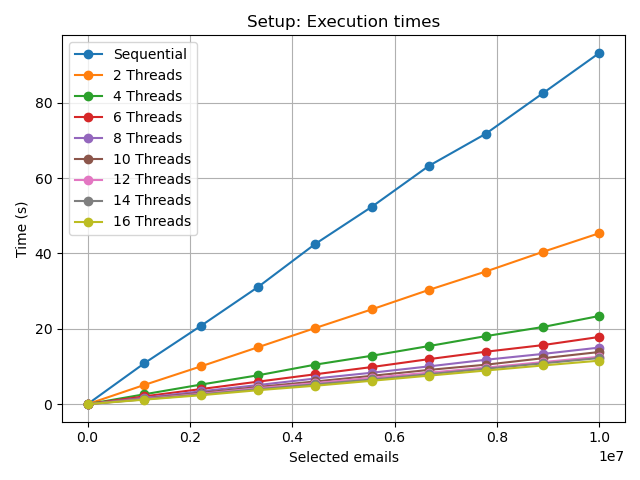
\includegraphics[width=\linewidth]{openmp/005/setup_times}
        \caption{Time setup Omp}\label{fig:005-setup_time_omp}
    \endminipage\hfill
    \minipage{0.49\textwidth}
    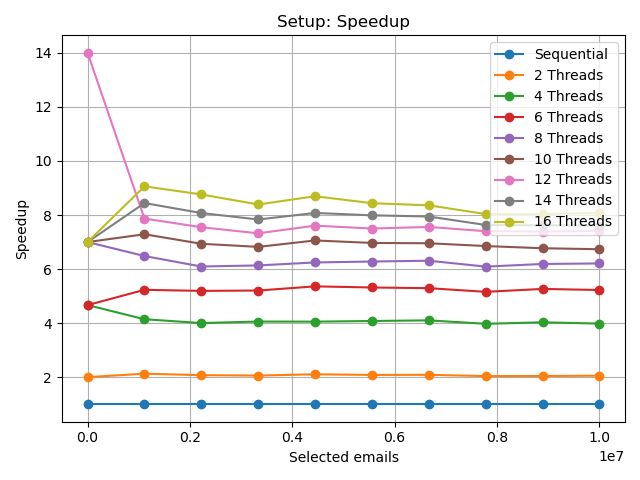
\includegraphics[width=\linewidth]{openmp/005/setup_speedup}
        \caption{Speedup setup Omp}\label{fig:005-setup_speedup_omp}
    \endminipage\hfill
\end{figure}
\begin{figure}[H]
    \centering
    \minipage{0.49\textwidth}
    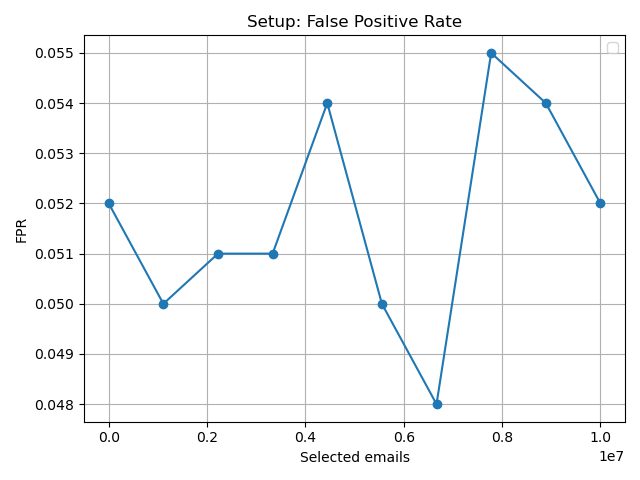
\includegraphics[width=\linewidth]{openmp/005/setup_fpr}
        \caption{FPR setup Omp}\label{fig:005-setup_fpr_omp}
    \endminipage\hfill
\end{figure}

Nella valutazione del tempo di esecuzione e dello speedup, è evidente come aumentando il numero di processi, il tempo
di esecuzione diminuisce in modo significativo rispetto alla versione sequenziale, raggiungendo un massimo di 9 con
l'utilizzo di 16 processi.
Possiamo notare come all'aumentare del numero di processi l'aumento dello speedup diminuisce, raggiungendo il valore di 8.
Per quanto riguarda il False Positive Rate, i valori ottenuti si aggirano molto intorno al valore di FPR
di 0.05 per il quale è stato configurato il BloomFilter.

\subsubsection{Filter}\label{subsubsec:fpr-005-filter}
\begin{figure}[H]
    \centering
    \minipage{0.49\textwidth}
    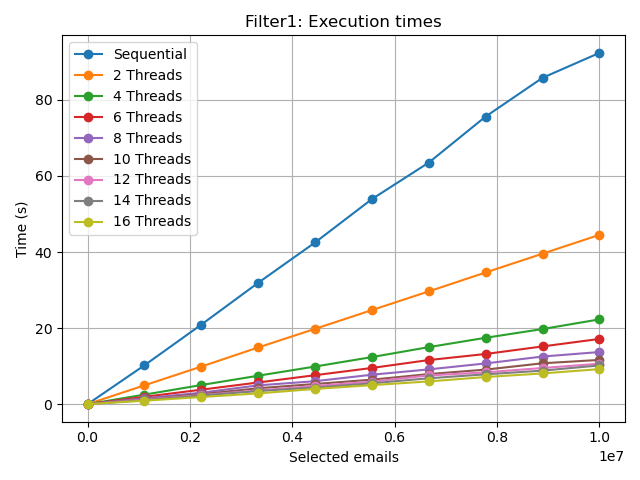
\includegraphics[width=\linewidth]{openmp/005/filter1_times}
        \caption{Time Filter Omp}\label{fig:005-filter_time_omp}
    \endminipage\hfill
    \minipage{0.49\textwidth}
    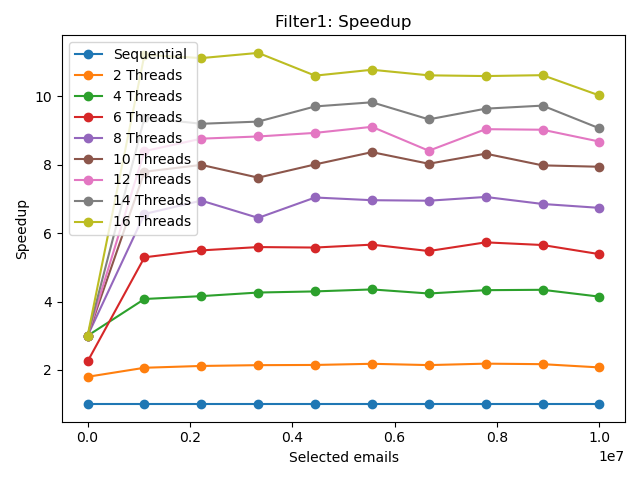
\includegraphics[width=\linewidth]{openmp/005/filter1_speedup}
        \caption{Speedup Filter Omp}\label{fig:005-filter_speedup_omp}
    \endminipage\hfill
\end{figure}
\begin{figure}[H]
    \centering
    \minipage{0.49\textwidth}
    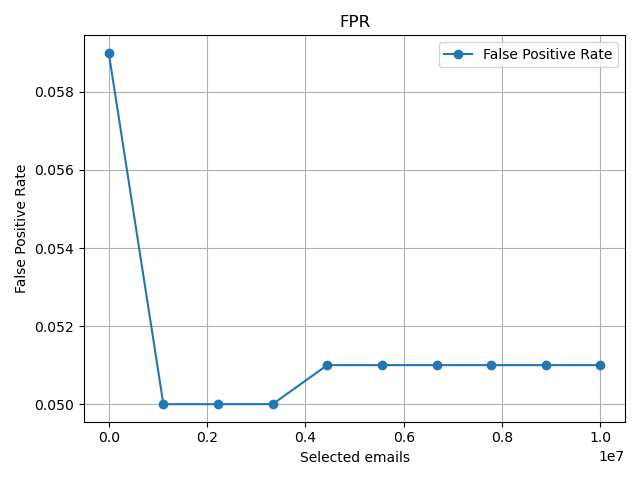
\includegraphics[width=\linewidth]{openmp/005/filter_fpr}
        \caption{FPR Filter Omp}\label{fig:005-filter_fpr_omp}
    \endminipage\hfill
\end{figure}

Come per la fase di setup, anche in questo caso, aumentando il numero di processi, il tempo di esecuzione diminuisce in
modo significativo rispetto alla versione sequenziale, raggiungendo un massimo di 11 con l'utilizzo di 16 processi.
In questo caso però, la variazione dello speedup non diminuisce in maniera più significativa rispetto alla fase di setup.
Il valore di FPR raggiunge il plateau una volta raggiunto un numero sufficiente di email.

\subsubsection{Confronto Filter}\label{subsubsec:confronto-filter}
Qui viene preso in considerazione le differenze tra le due versioni implementate del filtro.
\begin{figure}[H]
    \centering
    \minipage{0.49\textwidth}
    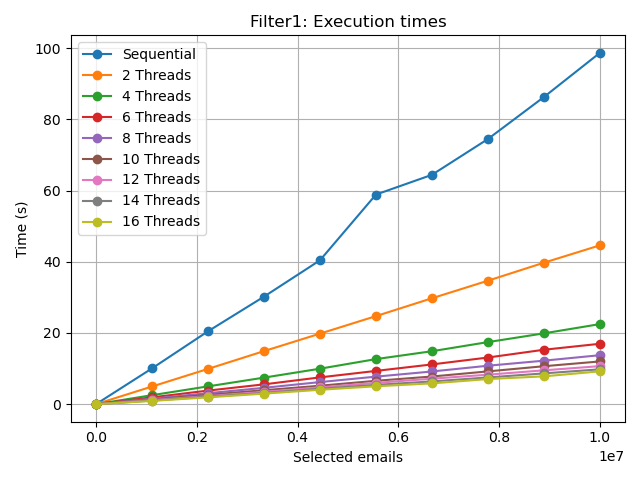
\includegraphics[width=\linewidth]{openmp/filters-005/filter1_times}
        \caption{Time Filter 1}\label{fig:005-filter1_time_omp}
    \endminipage\hfill
    \minipage{0.49\textwidth}
    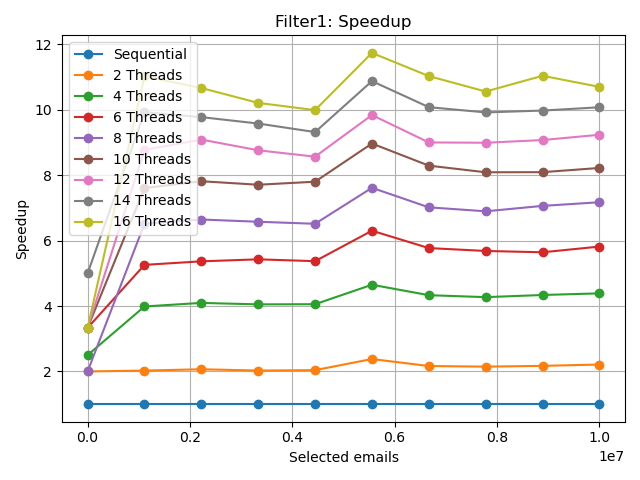
\includegraphics[width=\linewidth]{openmp/filters-005/filter1_speedup}
        \caption{Speedup Filter 1}\label{fig:005-filter1_speedup_omp}
    \endminipage\hfill
\end{figure}
\begin{figure}[H]
    \centering
    \minipage{0.49\textwidth}
    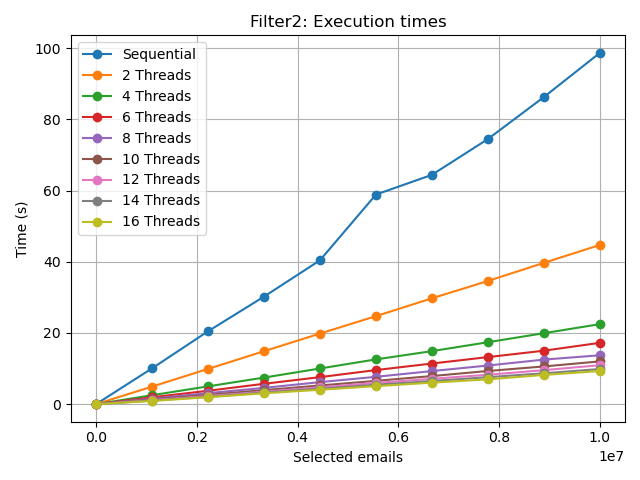
\includegraphics[width=\linewidth]{openmp/filters-005/filter2_times}
        \caption{Time Filter 2}\label{fig:005-filter2_time_omp}
    \endminipage\hfill
    \minipage{0.49\textwidth}
    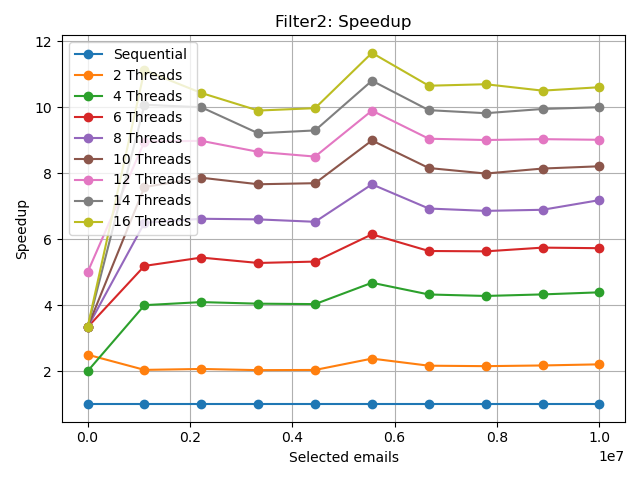
\includegraphics[width=\linewidth]{openmp/filters-005/filter2_speedup}
        \caption{Speedup Filter 2}\label{fig:005-filter2_speedup_omp}
    \endminipage\hfill
\end{figure}

Come è possibile notare, le due versioni del filtro presentano performance pressoché identiche in termini sia di tempo
di esecuzione che di speedup.

\subsection{Joblib}\label{subsec:joblib-test}
\subsubsection{Setup}\label{subsubsec:joblib-setup}
\begin{figure}[H]
    \centering
    \minipage{0.49\textwidth}
    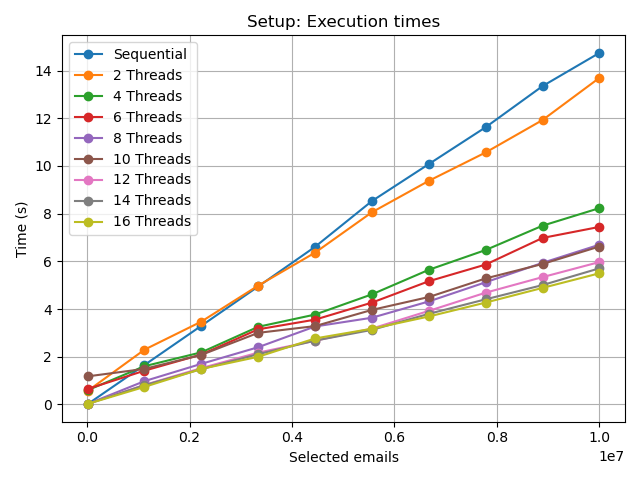
\includegraphics[width=\linewidth]{joblib/005/setup_time_plot}
        \caption{Time setup Joblib}\label{fig:005-setup_time_joblib}
    \endminipage\hfill
    \minipage{0.49\textwidth}
    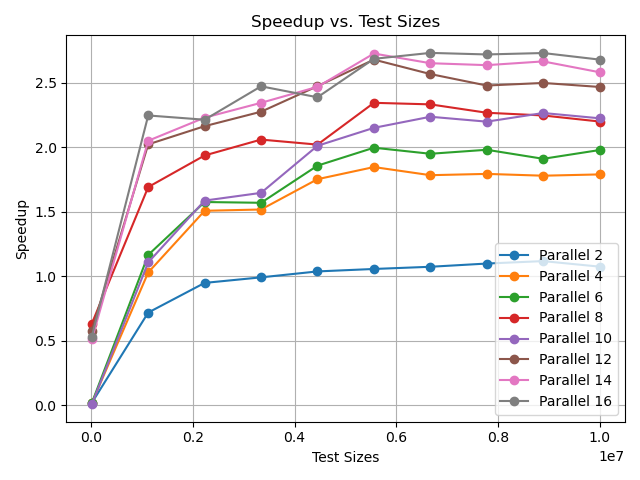
\includegraphics[width=\linewidth]{joblib/005/setup_speedup_plot}
        \caption{Speedup setup Joblib}\label{fig:005-setup_speedup_joblib}
    \endminipage\hfill
\end{figure}
\begin{figure}[H]
    \centering
    \minipage{0.49\textwidth}
    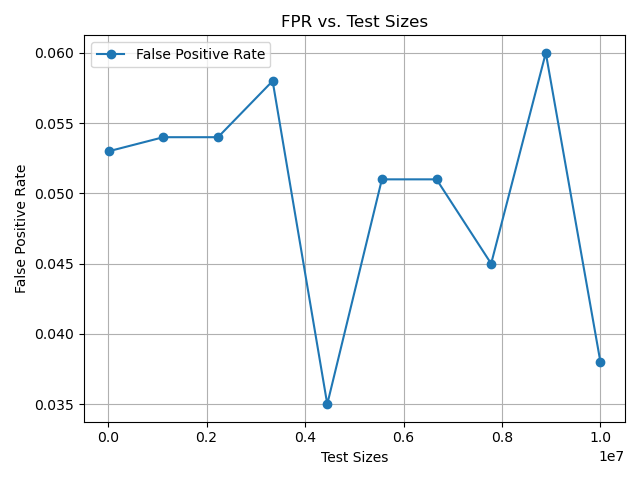
\includegraphics[width=\linewidth]{joblib/005/setup_fpr_plot}
        \caption{FPR setup Joblib}\label{fig:005-setup_fpr_joblib}
    \endminipage\hfill
\end{figure}

I risultati ottenuti con la versione Joblib mostrano come l'aumento del numero di processori

\subsubsection{Filter}\label{subsubsec:joblib-filter}
\begin{figure}
    \centering
    \minipage{0.49\textwidth}
    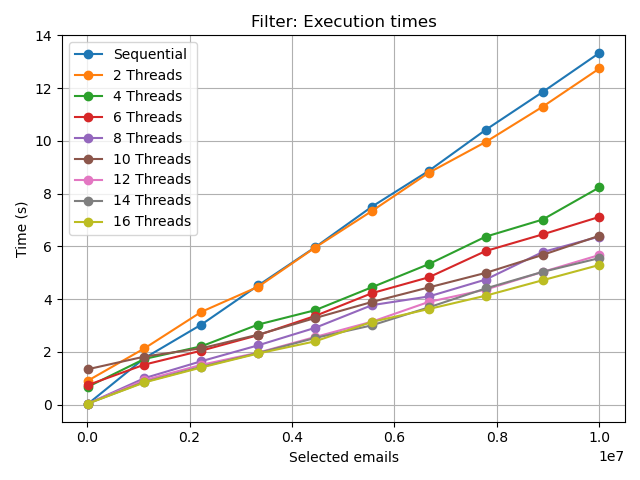
\includegraphics[width=\linewidth]{joblib/005/filter_time_plot}
        \caption{Time Filter Joblib}\label{fig:005-filter_time_joblib}
    \endminipage\hfill
    \minipage{0.49\textwidth}
    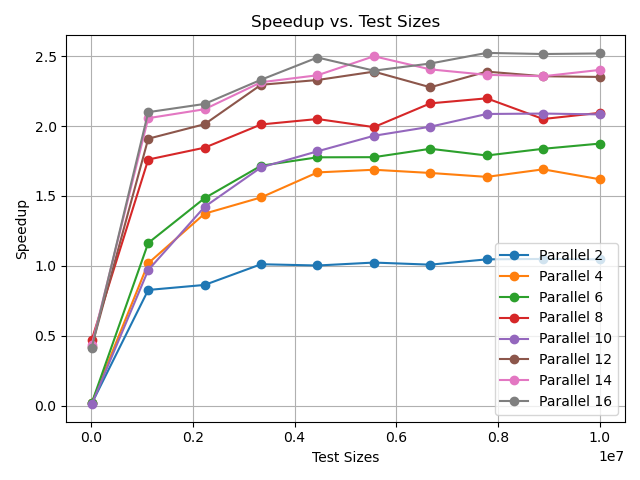
\includegraphics[width=\linewidth]{joblib/005/filter_speedup_plot}
        \caption{Speedup Filter Joblib}\label{fig:005-filter_speedup_joblib}
    \endminipage\hfill
\end{figure}
\begin{figure}[H]
    \centering
    \minipage{0.49\textwidth}
    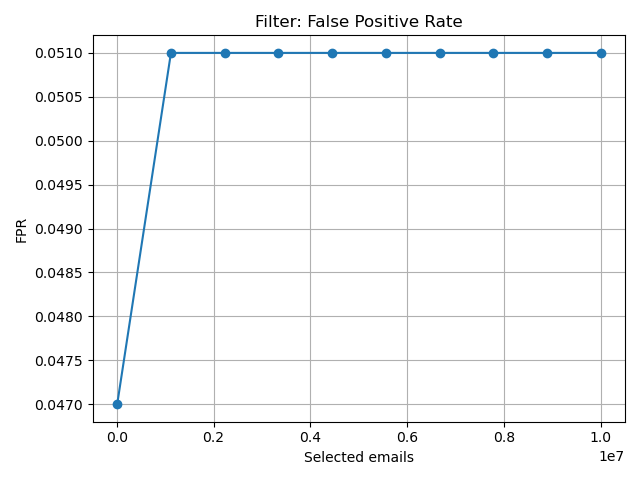
\includegraphics[width=\linewidth]{joblib/005/filter_fpr_plot}
        \caption{FPR Filter Joblib}\label{fig:005-filter_fpr_joblib}
    \endminipage\hfill
\end{figure}

\subsubsection{Chunks}\label{subsubsec:005-chunks}
Esploriamo ora l'opzione di eseguire un'operazione di chunking più ampia rispetto al numero di thread disponibili per
verificare se è possibile migliorare le performance, focalizzandoci esclusivamente sulla versione Joblib.
I valori di riferimento per i chunks sono 16, 32, 64, 128, 256, 512, 1024, 2048.

\begin{figure}[H]
    \centering
    \minipage{0.49\textwidth}
    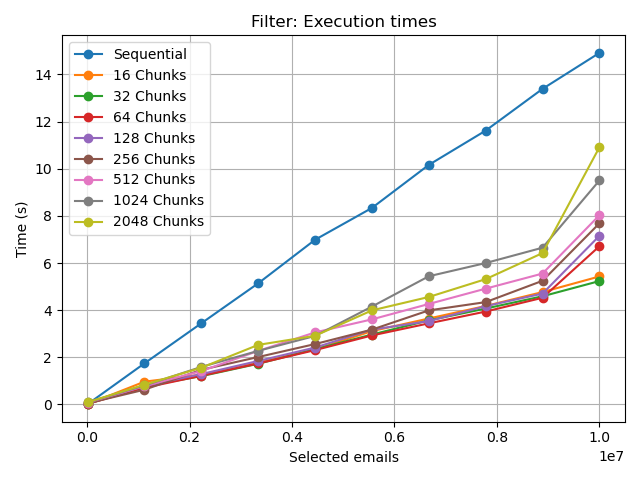
\includegraphics[width=\linewidth]{joblib/005/chunks_time_plot}
        \caption{Times setup Chunks}\label{fig:005-chunks_time}
    \endminipage\hfill
    \minipage{0.49\textwidth}
    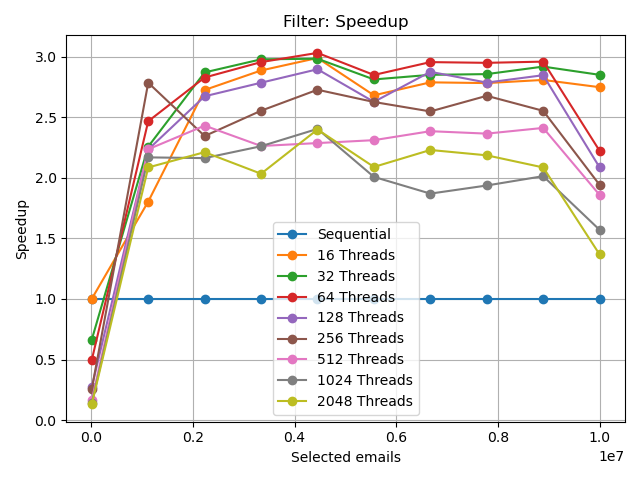
\includegraphics[width=\linewidth]{joblib/005/chunks_speedup_plot}
        \caption{Speedup setup Chunks}\label{fig:005-chunks_speedup}
    \endminipage\hfill
\end{figure}

I risultati ottenuti indicano che l'applicazione dell'operazione di chunking ha determinato miglioramenti
significativi nelle performance di speedup.
In particolare, l'aumento del numero di chunk ha contribuito a un miglioramento dello speedup,
raggiungendo un massimo di 3.
Tuttavia, oltre una soglia di 64 chunk, si è verificato un declino nelle performance.


\subsection{Confronto}\label{subsec:confronto}
Per il test di configurazione iniziale, è evidente che la versione sviluppata con OpenMP presenta una performance
temporale inferiore rispetto alla controparte.
Al contrario, in termini di speedup, la versione OpenMP supera la versione sviluppata con Joblib,
raggiungendo uno speedup massimo di 2.70 nella versione Joblib e 9 nella versione OpenMP, utilizzando il massimo
numero di thread disponibili.

I risultati massimi sono stati ottenuti sfruttando il numero massimo di thread disponibili.
Nel contesto della versione Joblib, i test iniziali con un numero più elevato di thread mostrano un tempo di esecuzione
peggiore rispetto alla versione sequenziale, probabilmente a causa del tempo di inizializzazione dei thread.
Nonostante l'aumento del numero di thread nella versione Joblib, lo speedup si stabilizza intorno al valore di 2.

Va notato che i valori di FPR (False Positive Rate) sono molto simili tra le due versioni.


Per il test di filtraggio, è evidente che la versione sviluppata con OpenMP presenta una performance temporale
inferiore rispetto alla sua controparte.
Tuttavia, in termini di speedup, la versione OpenMP supera la versione sviluppata con Joblib, raggiungendo un
massimo di 11 nella versione OpenMP e 2.5 nella versione Joblib, sfruttando il massimo numero di thread disponibili.

Anche in questo contesto, i valori di FPR (False Positive Rate) sono praticamente identici tra le due versioni.





    \clearpage
    \section{Conclusioni}\label{sec:conclusioni}
    I risultati ottenuti mostrano che la parallelizzazione delle operazioni di setup e filtraggio del BloomFilter
    consente di ottenere uno speedup significativo in relazione al numero di processori impiegati.
    Specificamente, in termini di tempo, la versione parallelizzata con Joblib è risultata più efficiente rispetto
    alla versione parallelizzata con Omp.
    Viceversa, la versione parallelizzata con Omp ha mostrato un miglioramento più significativo in termini di speedup.
    L'operazione di chunking ha permesso di ottenere uno speedup leggermente migliore rispetto alla versione senza chunking
    per alcuni valori di chunk size.

\end{document}